%\documentclass[hyperref={pdfpagelabels=false},slidetop,9pt]{beamer}
\documentclass[slidetop,8pt]{beamer}
\usepackage[T1]{fontenc}
\usepackage[utf8]{inputenc}
\newcommand{\id}{54}
\newcommand{\nom}{Liaisons mécaniques}
\newcommand{\sequence}{04}
\newcommand{\num}{01}
\newcommand{\type}{TP}
\newcommand{\descrip}{Modélisation d'un solide. Comportement des liaisons mécaniques. Modéliser les mécanismes du laboratoire par un schéma cinématique, paramétré.}
\newcommand{\competences}{A3-C4: Analyse d'architecture et de comportement \\ &  Mod1-C1: Isolement d'un solide ou d'un système de solides \\ &  Mod2-C10-1: Modèle de solide indéformable \\ &  Mod2-C11: Modélisation géométrique et cinématique des mouvements entre solides indéformables \\ &  Mod2-C12: Modélisation cinématique des liaisons entre solides \\ &  Mod2-C15: Modélisation des actions mécaniques \\ &  Rés-C6: Utilisation d'un solveur ou d'un logiciel multi physique \\ &  Com1-C1: Différents descripteurs introduits dans le programme \\ &  Com2-C4: Outils de communication}
\newcommand{\nbcomp}{9}
\newcommand{\systemes}{Plateforme Stewart}
\newcommand{\systemessansaccent}{Plateforme Stewart}
\newcommand{\ilot}{2}
\newcommand{\ilotstr}{02}
\newcommand{\dossierilot}{\detokenize{Ilot_02 Plateforme Stewart}}
\newcommand{\imageun}{Plateforme}

\newcommand{\urlsysteme}{\href{https://www.costadoat.fr/systeme/57}{Ressources système}}
\newcommand{\matlabsimscape}{\href{https://github.com/Costadoat/Sciences-Ingenieur/raw/master/Systemes/Plateforme Stewart/Plateforme_Stewart_Simscape.zip}{Modèle Simscape}}
\newcommand{\solidworks}{\href{https://github.com/Costadoat/Sciences-Ingenieur/raw/master/Systemes/Plateforme Stewart/Plateforme_Stewart_Solidworks.zip}{Modèle Solidworks}}
\newcommand{\edrawings}{\href{https://github.com/Costadoat/Sciences-Ingenieur/raw/master/Systemes/Plateforme Stewart/Plateforme_Stewart.EASM}{Modèle eDrawings}}
\newcommand{\test}{Stewart_param1}
\newcommand{\testi}{Stewart_param2}
\newcommand{\testii}{Stewart_param3}
\newcommand{\testiii}{Stewart_param4}
\newcommand{\testiiii}{Stewart_euler}
\usepackage{etex}
\usepackage{tikz}
\usepackage[european]{circuitikz}
\usepackage{pgf}
\usepackage[all]{xy}
\usepackage{pgfpages}
\usepackage{graphbox}
\usepackage{pdfpages}
\usepackage[adobe-utopia]{mathdesign}
\usepackage{ifthen}
\usepackage{cancel}
\usepackage{framed}
\usepackage{subfig}
\usepackage{tabularx}
\usepackage{setspace}
\usepackage{soul}
\usepackage{schemabloc}
\usepackage{eqnarray}
\usepackage[dot, phantomtext]{dashundergaps}
\usepackage{media9}
\usepackage{multimedia}
\usepackage{textcomp}

\author{Renaud Costadoat}
\institute{Lycée Dorian}

\usepackage{multido}
\usepackage{multirow}
\usepackage{multicol} % Portions de texte en colonnes
\usepackage{flafter}%floatants après la référence

\usepackage{color}
\usepackage{xcolor}
\usepackage{colortbl}

\usepackage[gen]{eurosym}
\usepackage{tikz}
%\usepackage{pstricks,pst-node,pst-tree,pst-solides3d}
\usepackage{lmodern}
\usepackage[francais]{babel}
\usepackage{pslatex}
\usetheme{renaud}
\usepackage{times}
\usepackage{amsmath}
\usepackage{verbatim}
\usepackage{moreverb}
%\usetikzlibrary{arrows,shapes}
\usepackage{graphicx}
\usepackage{psfrag}
\usepackage{wrapfig}
\usepackage{etoolbox}

\definecolor{gris25}{gray}{0.75}
\definecolor{bleu}{RGB}{18,33,98}
\definecolor{bleuf}{RGB}{42,94,171}
\definecolor{bleuc}{RGB}{231,239,247}
\definecolor{rougef}{RGB}{185,18,27}
\definecolor{rougec}{RGB}{255,188,204}%255,230,231
\definecolor{vertf}{RGB}{103,126,82}
\definecolor{vertc}{RGB}{220,255,191}

\setlength\parindent{24pt}
\parskip 7.2pt
\parindent 8pt

\newenvironment{rem}[1][\hsize]%
{%
    \def\FrameCommand
   {%
\rotatebox{90}{\textit{\textsf{Remarque}}} 
       {\color{bleuf}\vrule width 3pt}%
       \hspace{0pt}%must no space.
       \fboxsep=\FrameSep\colorbox{bleuc}%
  }%
    \MakeFramed{\hsize#1\advance\hsize-\width\FrameRestore}%
}%
{\endMakeFramed}%


\newenvironment{savoir}[1][\hsize]%
{%
    \def\FrameCommand
    {%
\rotatebox{90}{\textit{\textsf{Savoir}}} 
        {\color{bleuf}\vrule width 3pt}%
        \hspace{0pt}%must no space.
        \fboxsep=\FrameSep\colorbox{bleuc}%
    }%
    \MakeFramed{\hsize#1\advance\hsize-\width\FrameRestore}%
}%
{\endMakeFramed}%

\newenvironment{prob}[1][\hsize]%
{%
    \def\FrameCommand%
    {%
\rotatebox{90}{\textit{\textsf{Problematique}}} 
        {\color{rougef}\vrule width 3pt}%
        \hspace{0pt}%must no space.
        \fboxsep=\FrameSep\colorbox{rougec}%
    }%
    \MakeFramed{\hsize#1\advance\hsize-\width\FrameRestore}%
}%
{\endMakeFramed}%

\newenvironment{obj}[1][\hsize]%
{%
    \def\FrameCommand%
    {%
\rotatebox{90}{\textit{\textsf{Objectif}}} 
        {\color{vertf}\vrule width 3pt}%
        \hspace{0pt}%must no space.
        \fboxsep=\FrameSep\colorbox{vertc}%
    }%
    \MakeFramed{\hsize#1\advance\hsize-\width\FrameRestore}%
}%
{\endMakeFramed}%

\newenvironment{defi}[1][\hsize]%
{%
    \def\FrameCommand%
    {%
\rotatebox{90}{\textit{\textsf{Definition}}} 
        {\color{bleuf}\vrule width 3pt}%
        \hspace{0pt}%must no space.
        \fboxsep=\FrameSep\colorbox{rougec}%
    }%
    \MakeFramed{\hsize#1\advance\hsize-\width\FrameRestore}%
}%
{\endMakeFramed}%


\newenvironment{hypo}[1][\hsize]%
{%
    \def\FrameCommand%
    {%
\rotatebox{90}{\textit{\textsf{Hypothèse\\}}} 
        {\color{bleuf}\vrule width 3pt}%
        \hspace{0pt}%must no space.
        \fboxsep=\FrameSep\colorbox{bleuc}%
    }%
    \MakeFramed{\hsize#1\advance\hsize-\width\FrameRestore}%
}%
{\endMakeFramed}%


\newenvironment{prop}[1][\hsize]%
{%
    \def\FrameCommand%
    {%
\rotatebox{90}{\textit{\textsf{Propriété}}} 
        {\color{bleuf}\vrule width 3pt}%
        \hspace{0pt}%must no space.
        \fboxsep=\FrameSep\colorbox{bleuc}%
    }%
    \MakeFramed{\hsize#1\advance\hsize-\width\FrameRestore}%
}%
{\endMakeFramed}%

\newenvironment{props}[1][\hsize]%
{%
    \def\FrameCommand%
    {%
\rotatebox{90}{\textit{\textsf{Propriétés}}} 
        {\color{bleuf}\vrule width 3pt}%
        \hspace{0pt}%must no space.
        \fboxsep=\FrameSep\colorbox{bleuc}%
    }%
    \MakeFramed{\hsize#1\advance\hsize-\width\FrameRestore}%
}%
{\endMakeFramed}%

\newenvironment{exemple}[1][\hsize]%
{%
    \def\FrameCommand%
    {%
\rotatebox{90}{\textit{\textsf{Exemple}}} 
        {\color{vertf}\vrule width 3pt}%
        \hspace{0pt}%must no space.
        \fboxsep=\FrameSep\colorbox{vertc}%
    }%
    \MakeFramed{\hsize#1\advance\hsize-\width\FrameRestore}%
}%
{\endMakeFramed}%

\newenvironment{resultat}[1][\hsize]%
{%
    \def\FrameCommand%
    {%
\rotatebox{90}{\textit{\textsf{Résultat}}} 
        {\color{rougef}\vrule width 3pt}%
%        {\color{bleuf}\vrule width 3pt}%
        \hspace{0pt}%must no space.
        \fboxsep=\FrameSep\colorbox{rougec}%
    }%
    \MakeFramed{\hsize#1\advance\hsize-\width\FrameRestore}%
}%
{\endMakeFramed}%

\newenvironment{methode}[1][\hsize]%
{%
    \def\FrameCommand%
    {%
\rotatebox{90}{\textit{\textsf{Méthode\\}}} 
        {\color{rougef}\vrule width 3pt}%
        \hspace{0pt}%must no space.
        \fboxsep=\FrameSep\colorbox{rougec}%
    }%
    \MakeFramed{\hsize#1\advance\hsize-\width\FrameRestore}%
}%
{\endMakeFramed}%

\newenvironment{theo}[1][\hsize]%
{%
    \def\FrameCommand%
    {%
\rotatebox{90}{\textit{\textsf{Théorème\\}}} 
        {\color{rougef}\vrule width 3pt}%
        \hspace{0pt}%must no space.
        \fboxsep=\FrameSep\colorbox{rougec}%
    }%
    \MakeFramed{\hsize#1\advance\hsize-\width\FrameRestore}%
}%
{\endMakeFramed}%

\newenvironment{warn}[1][\hsize]%
{%
    \def\FrameCommand%
    {%
\rotatebox{90}{\textit{\textsf{Attention\\}}} 
        {\color{rougef}\vrule width 3pt}%
        \hspace{0pt}%must no space.
        \fboxsep=\FrameSep\colorbox{rougec}%
    }%
    \MakeFramed{\hsize#1\advance\hsize-\width\FrameRestore}%
}%
{\endMakeFramed}%

% \usepackage{pstricks}
%\usepackage{minitoc}
% \setcounter{minitocdepth}{4}

\setcounter{tocdepth}{2}

% \mtcselectlanguage{french} 

%\usepackage{draftcopy}% "Brouillon"
% \usepackage{floatflt}
\usepackage{psfrag}
%\usepackage{listings} % Permet d'insérer du code de programmation
\renewcommand{\baselinestretch}{1.2}

% Changer la num�rotation des figures :
% ------------------------------------
% \makeatletter
% \renewcommand{\thefigure}{\ifnum \c@section>\z@ \thesection.\fi
%  \@arabic\c@figure}
% \@addtoreset{figure}{section}
% \makeatother
 


%%%%%%%%%%%%
% Définition des vecteurs %
%%%%%%%%%%%%
 \newcommand{\vect}[1]{\overrightarrow{#1}}

%%%%%%%%%%%%
% Définition des torseusr %
%%%%%%%%%%%%

 \newcommand{\torseur}[1]{%
\left\{{#1}\right\}
}

\newcommand{\torseurcin}[3]{%
\left\{\mathcal{#1} \left(#2/#3 \right) \right\}
}

\newcommand{\torseurstat}[3]{%
\left\{\mathcal{#1} \left(#2\rightarrow #3 \right) \right\}
}

 \newcommand{\torseurc}[8]{%
%\left\{#1 \right\}=
\left\{
{#1}
\right\}
 = 
\left\{%
\begin{array}{cc}%
{#2} & {#5}\\%
{#3} & {#6}\\%
{#4} & {#7}\\%
\end{array}%
\right\}_{#8}%
}

 \newcommand{\torseurcol}[7]{
\left\{%
\begin{array}{cc}%
{#1} & {#4}\\%
{#2} & {#5}\\%
{#3} & {#6}\\%
\end{array}%
\right\}_{#7}%
}

 \newcommand{\torseurl}[3]{%
%\left\{\mathcal{#1}\right\}_{#2}=%
\left\{%
\begin{array}{l}%
{#1} \\%
{#2} %
\end{array}%
\right\}_{#3}%
}

 \newcommand{\vectv}[3]{%
\vect{V\left( {#1} \in {#2}/{#3}\right)}
}


\newcommand{\vectf}[2]{%
\vect{R\left( {#1} \rightarrow {#2}\right)}
}

\newcommand{\vectm}[3]{%
\vect{\mathcal{M}\left( {#1}, {#2} \rightarrow {#3}\right)}
}


 \newcommand{\vectg}[3]{%
\vect{\Gamma \left( {#1} \in {#2}/{#3}\right)}
}

 \newcommand{\vecto}[2]{%
\vect{\Omega\left( {#1}/{#2}\right)}
}

\newcommand{\reponse}[1][4]
{
\multido{}{#1}
{
\begin{center}
\makebox[0.9\linewidth]{\dotfill} \end{center}
}}


% }$$\left\{\mathcal{#1} \right\}_{#2} =%
% \left\{%
% \begin{array}{c}%
%  #3 \\%
%  #4 %
% \end{array}%
% \right\}_{#5}}


%  ------------------------------------------
% | Modification du formatage des sections : | 
%  ------------------------------------------

% Grands titres :
% ---------------

\newcommand{\titre}[1]{%
\begin{center}
      \bigskip
      \rule{\textwidth}{1pt}
      \par\vspace{0.1cm}
      
      \textbf{\large #1}
      \par\rule{\textwidth}{1pt}
    \end{center}
    \bigskip
  }

% Supprime le numéro du chapitre dans la numérotation des sections:
% -----------------------------------------------------------------
\makeatletter
\renewcommand{\thesection}{\@arabic\c@section}
\makeatother


% \titleformat{\chapter}[display]
% {\normalfont\Large\filcenter}
% {}
% {1pc}
% {\titlerule[1pt]
%   \vspace{1pc}%
%   \Huge}[\vspace{1ex}%
% \titlerule]


%%%% Chapitres Comme PY Pechard %%%%%%%%%
% numéro du chapitre
\DeclareFixedFont{\chapnumfont}{OT1}{phv}{b}{n}{80pt}
% pour le mot " Chapitre "
\DeclareFixedFont{\chapchapfont}{OT1}{phv}{m}{it}{40pt}
% pour le titre
\DeclareFixedFont{\chaptitfont}{T1}{phv}{b}{n}{25pt}

\definecolor{gris}{gray}{0.75}
\setbeamertemplate{section in toc}[sections numbered]

\newlength{\RoundedBoxWidth}
\newsavebox{\GrayRoundedBox}
\newenvironment{GrayBox}[1][\dimexpr\textwidth-4.5ex]%
   {\setlength{\RoundedBoxWidth}{\dimexpr#1}
    \begin{lrbox}{\GrayRoundedBox}
       \begin{minipage}{\RoundedBoxWidth}}%
   {   \end{minipage}
    \end{lrbox}
    \begin{center}
    \begin{tikzpicture}%
       \draw node[draw=bleuf,fill=bleuc,rounded corners,%
             inner sep=2ex,text width=\RoundedBoxWidth]%
             {\usebox{\GrayRoundedBox}};
    \end{tikzpicture}
    \end{center}}
    
\ifdef{\prive}{\pgfpagesuselayout{2 on 1}[a4paper,border shrink=0mm]}
\ifdef{\prive}{\setbeamertemplate{navigation symbols}{}}
\setbeamertemplate{itemize item}[ball]
%\setbeamertemplate{blocks}[rounded]%[shadow=true]
\setbeamercolor{block title}{fg=white,bg=grisf}        % titre block normal 
\setbeamercolor{block body}{fg=grisf,bg=grisc!50}      % corps block normal
\setbeamercolor{block body alerted}{fg=white,bg=warning}   % idem pour un block alerte

\title{\nom}
\date{S\sequence \ - \type\num}

\begin{document}
\shorthandoff{:!}
\bibliographystyle{abbrvnat-fr}

\usebackgroundtemplate%
{%
    \centering
\includegraphics[width=\paperwidth]{../../img/fond2}%
}

{
\setbeamertemplate{navigation symbols}{}
\setbeamertemplate{headline}[pagetitre]
\setbeamertemplate{footline}[pagetitre]
\usebackgroundtemplate{\centering
\includegraphics[width=\paperwidth]{../../img/fond}}
\frame{\titlepage}
}



\section{Vecteur}

{\frame{
\frametitle{Introduction}

\begin{savoir}
Vous êtes capables :
\begin{itemize}
 \item de résoudre des équations différentielles à l'aide des transformées de Laplace,
 \item de représenter des réponses impulsionnelles et indicielles,
 \item de représenter un SLCI à l'aide d'un schéma blocs. 
\end{itemize}
\end{savoir}

\begin{prob}
Vous devez êtes capables :
 \begin{itemize}
 \item de déterminer la loi entrée/sortie d'une chaîne de transmission,
 \item de modéliser la géométrie d'un système.
 \end{itemize}
\end{prob}
}}

{\frame{
\frametitle{Introduction mathématique}

\begin{obj}
La mécanique a pour objet l'étude du \textbf{mouvement}, des déformations ou des états d'équilibre des systèmes physiques.

Afin d'appréhender la \textbf{modélisation} et la \textbf{résolution} de ces problèmes il est nécessaire de revoir les notions de mathématique suivantes:

\begin{itemize}
 \item le vecteur,
 \item le produit scalaire,
 \item le produit vectoriel,
 \item le champ de vecteurs,
 \item le torseur,
 \item les repères et axes de coordonnées.
\end{itemize}
\end{obj}
}}


{\frame{
\frametitle{Vecteur}

\begin{minipage}{0.7\linewidth}
	\begin{defi}
	Un vecteur non nul $\overrightarrow{AB}$ est caractérisé par : 
	\begin{itemize}
	 \item \ifdef{\public}{sa \textbf{direction}}{.................} : la droite $(D)$ passant par $A$ et $B$, 
	 \item \ifdef{\public}{son \textbf{sens}}{.................} : de $A$ vers $B$,
	 \item \ifdef{\public}{sa \textbf{norme}}{.................} : la distance $d$ entre les points $A$ et $B$.
	\end{itemize}
	\end{defi}
\end{minipage}
\hfill
\begin{minipage}{0.25\linewidth}
\ifdef{\public}{\centering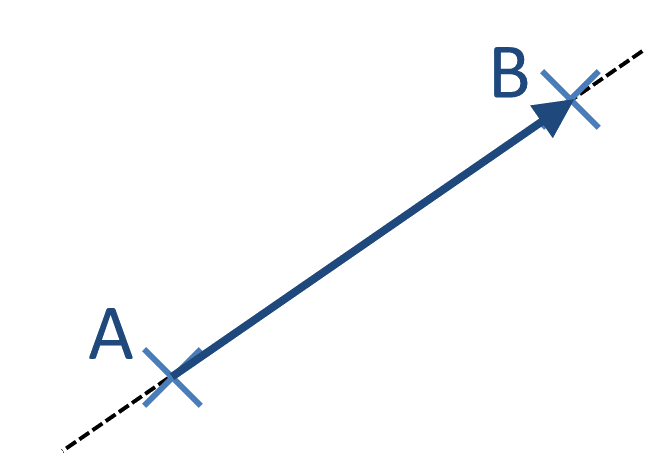
\includegraphics[width=0.9\linewidth]{img/vecteur}}{}
\end{minipage}

\vfill

\begin{itemize}
 \item \textbf{Vecteur glissant:} Un vecteur glissant (ou glisseur) est défini par une droite $(D)$ et un vecteur $\overrightarrow{V}$. Deux vecteurs glissants sont équivalents s'ils ont même support et même vecteur représentant. 
 \item \textbf{Vecteur lié:} Un vecteur lié est défini par une origine A et un vecteur $\overrightarrow{V}$.
\end{itemize}
}}

{\frame{
\frametitle{Composantes d'un vecteur}

\begin{itemize}
 \item \textbf{Repère orthonormé direct}: Un repère orthonormé direct de dimension 3, (R), est constitué d'une base orthonormée directe de dimension 3.
\end{itemize}


\begin{center}
\begin{minipage}{0.4\linewidth}
Elle est définie par trois vecteurs unitaires (de norme 1) $\overrightarrow{x}$, $\overrightarrow{y}$, $\overrightarrow{z}$ tels que $\overrightarrow{x}.\overrightarrow{y}=0$ et $\overrightarrow{z}=\overrightarrow{x}\wedge\overrightarrow{y}$, soit son origine $O$, on le note : $R(O,\overrightarrow{x},\overrightarrow{y},\overrightarrow{z})$.
\end{minipage}
\hfill
\begin{minipage}{0.56\linewidth}
\begin{tabular}{p{3.5cm}p{2cm}}
{\small Plan} & {\small Spatial} \\
\ifdef{\public}{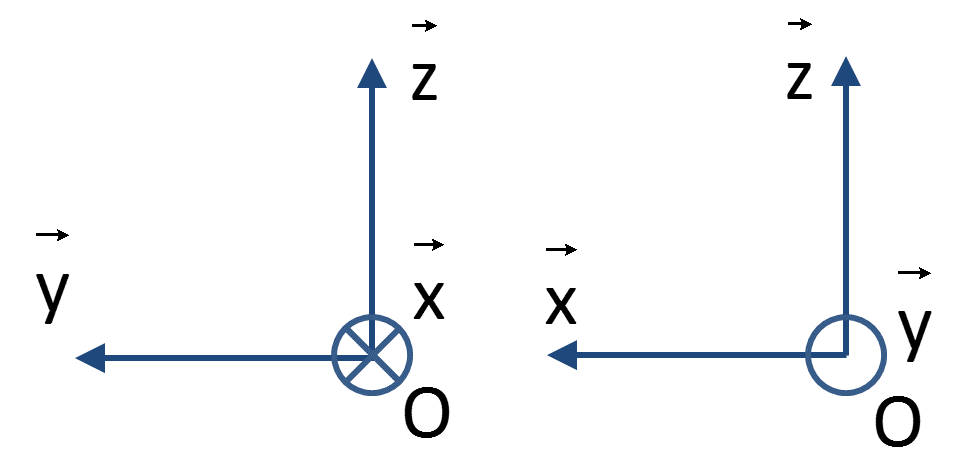
\includegraphics[width=\linewidth]{img/repere1} &
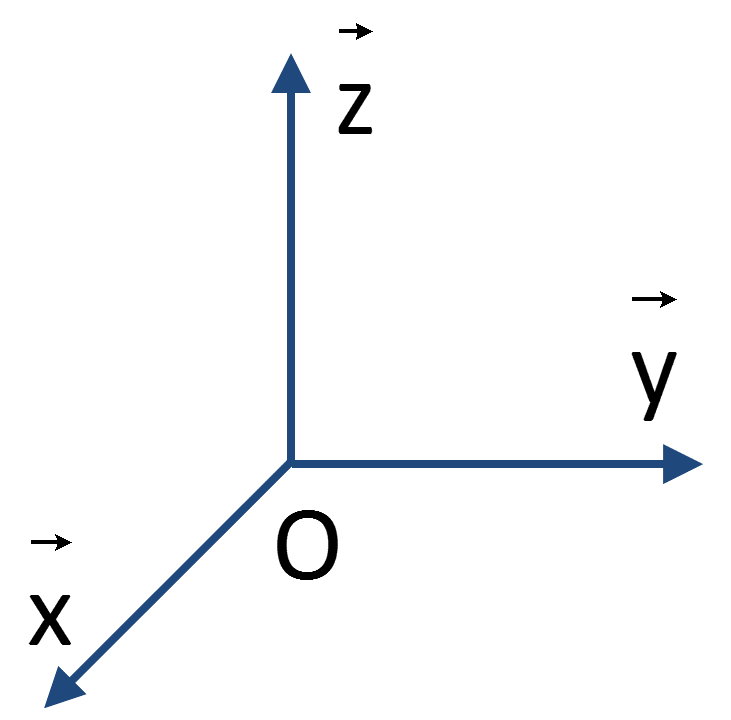
\includegraphics[width=\linewidth]{img/repere2} \\}{ \vspace{1cm} & \vspace{1cm}}
\end{tabular}
\end{minipage}
\end{center}

\begin{minipage}{0.48\linewidth}
\begin{itemize}
 \item Soit un point $M$, sa position dans $R(O,\overrightarrow{x},\overrightarrow{y},\overrightarrow{z})$ est le vecteur $\overrightarrow{OM}$,
 \item $\overrightarrow{OM}=dx.\overrightarrow{x}+dy.\overrightarrow{y}+dz.\overrightarrow{z}$.
 \item Écriture en colonne: $\overrightarrow{OM}=\left[\begin{array}{c}dx \\ dy \\ dz \end{array}\right]$
 \item Norme: $\|\overrightarrow{OM}\|=\sqrt{dx^2+dy^2+dz^2}$
\end{itemize}
\end{minipage}
\hfill
\begin{minipage}{0.48\linewidth}
\centering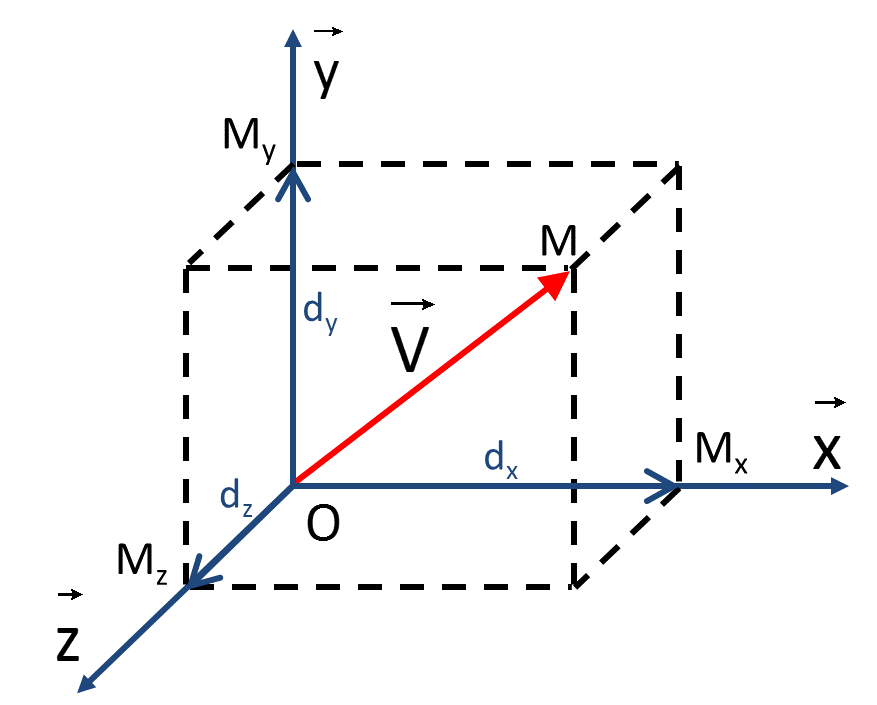
\includegraphics[width=0.8\linewidth]{img/repere3}
\end{minipage}
}}

{\frame{
\frametitle{Produit d'un vecteur par un scalaire}

Le terme \textbf{scalaire} désigne ici un nombre réel. Le produit d'un vecteur $\overrightarrow{u}$ par un scalaire $a$ est un vecteur noté : $a.\overrightarrow{u}$.
\begin{itemize}
 \item de même direction et sens que $\overrightarrow{u}$, dont la longueur vaut: $a.\|\overrightarrow{u}\|$, si $a>0$,
 \item de même direction mais de sens contraire que $\overrightarrow{u}$, dont la longueur vaut : $-a.\|\overrightarrow{u}\|$, si a < 0,
 \item il s'agit d'un vecteur nul si a = 0. 
\end{itemize}

\begin{center}
 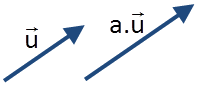
\includegraphics[width=0.2\linewidth]{img/vecteur2}
\end{center}

Le produit d'un vecteur par un scalaire est \textbf{distributif} sur l'addition des scalaires :
$(a+b).\overrightarrow{u}=a.\overrightarrow{u}+b.\overrightarrow{u}$ mais il n'est pas commutatif : la notation $\overrightarrow{u}.a$ n'a pas de sens.

Remarque : deux vecteurs sont colinéaires (parallèles) si et seulement s'ils sont proportionnels, c'est-à-dire s'il existe un nombre $a$ tel que $\overrightarrow{u}=a.\overrightarrow{v}$.
}}

{\frame{
\frametitle{Somme de deux vecteurs}

\begin{minipage}{0.76\linewidth}
La somme de deux vecteurs $\overrightarrow{u}$ et $\overrightarrow{v}$ est un vecteur, noté $\overrightarrow{u}+\overrightarrow{v}$, qui est construit de la manière suivante :
\begin{itemize}
 \item on amène l'origine du deuxième vecteur à l'extrémité du premier
 \item la somme est le vecteur qui joint l'origine du premier vecteur à l'extrémité de second
 \item il s'agit du troisième côté d'un triangle formé par les deux premiers vecteurs
\end{itemize}
\end{minipage}
\hfill
\begin{minipage}{0.2\linewidth}
\centering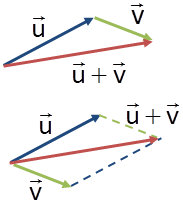
\includegraphics[width=\linewidth]{img/vecteur3}
\end{minipage}

\vfill

\begin{defi}
A partir de trois points A, B et C existe la relation de \textbf{Chasles}: \ifdef{\public}{$\overrightarrow{AB}+\overrightarrow{BC}=\overrightarrow{AC}$}{..................................} \\
Cela permet d'introduire les vecteurs opposés: $-\overrightarrow{AB}=\overrightarrow{BA}$
\end{defi}

En effet, $\overrightarrow{AB}+\overrightarrow{BA}=\overrightarrow{AA}=\overrightarrow{0}$, donc $-\overrightarrow{AB}=\overrightarrow{BA}$.

Le produit d'un scalaire par un vecteur est distributif sur l'addition des vecteurs : $a.(\overrightarrow{u}+\overrightarrow{v})=a.\overrightarrow{u}+a.\overrightarrow{v}$
}}

{\frame{
\frametitle{Produit scalaire de deux vecteurs}

\begin{defi}
Si $\overrightarrow{u}$ et $\overrightarrow{v}$ sont deux vecteurs faisant un angle géométrique $\alpha$, le produit scalaire noté $\overrightarrow{u}.\overrightarrow{v}$, le nombre réel valant: \ifdef{\public}{$\overrightarrow{u}.\overrightarrow{v}=\|\overrightarrow{u}\|.\|\overrightarrow{v}\|.cos(\alpha)$.}{.......................................}
\end{defi}

\begin{minipage}[t]{0.3\linewidth}
Le produit scalaire est nul
\end{minipage}\hfill
\begin{minipage}[t]{0.67\linewidth}
\begin{itemize}
 \item Si l'un des vecteurs est nul
 \item Si l'angle entre eux est droit (c'est-à-dire si et $\alpha=\frac{\pi}{2}rad=90\textdegree$),
 \item Les vecteurs $\overrightarrow{u}$ et $\overrightarrow{v}$ sont dans ce cas orthogonaux.
\end{itemize}
\end{minipage}

Le produit scalaire strictement positif si l'angle est aigu et strictement négatif si l'angle est obtus. Dans les cas suivants, $\overrightarrow{u}.\overrightarrow{v}=v_u.\|\overrightarrow{u}\|=u_v.\|\overrightarrow{v}\|$.

\begin{center}
 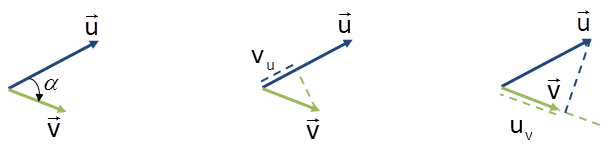
\includegraphics[width=0.6\linewidth]{img/vecteur4}
\end{center}
}}

{\frame{
\frametitle{Propriétés du produit scalaire de deux vecteurs}

\begin{itemize}
 \item Le produit scalaire est commutatif $\overrightarrow{u}.\overrightarrow{v}=\overrightarrow{v}.\overrightarrow{u}$,
 \item Il est distributif sur l'addition des vecteurs $\overrightarrow{u}.(\overrightarrow{v}+\overrightarrow{w})=\overrightarrow{u}.\overrightarrow{v}+\overrightarrow{u}.\overrightarrow{w}$,
 \item Le vecteur nul est l'élément absorbant du produit scalaire $\overrightarrow{u}.\overrightarrow{0}=\overrightarrow{0}.\overrightarrow{u}=0$,
 \item $\overrightarrow{u}.\overrightarrow{u}$ s'appelle le carré scalaire du vecteur $\overrightarrow{u}$ et se note $\overrightarrow{u}^2$, ainsi $\overrightarrow{u}^2=\overrightarrow{u}.\overrightarrow{u}$,
 \item Le carré scalaire d'un vecteur est égal au carré de sa norme $\overrightarrow{u}^2=\|\overrightarrow{u}\|^2$ et donc $\sqrt{\overrightarrow{u}^2}=\|\overrightarrow{u}\|$,
 \item Deux vecteurs non nuls sont orthogonaux si et seulement si leur produit scalaire est nul, $\overrightarrow{u}$ est perpendiculaire à $\overrightarrow{v}$ si et seulement si $\overrightarrow{u}.\overrightarrow{v}=0$,
 \item Dans le plan rapporté à une base orthonormale ($\overrightarrow{i},\overrightarrow{j}$),\\
 $\overrightarrow{u}.\overrightarrow{v}=u_x.v_x+u_y.v_y$
 \item Dans le plan rapporté à une base orthonormale ($\overrightarrow{i},\overrightarrow{j},\overrightarrow{k}$),\\
 $\overrightarrow{u}.\overrightarrow{v}=u_x.v_x+u_y.v_y+u_z.v_z$
\end{itemize}
}}

{\frame{
\frametitle{Produit vectoriel de deux vecteurs}

\begin{defi}
Le produit vectoriel des deux vecteurs $\overrightarrow{u}$ et $\overrightarrow{v}$, noté $\overrightarrow{u}\wedge\overrightarrow{v}$, est un vecteur:
\begin{itemize}
 \item normal au plan vectoriel de base $(\overrightarrow{u},\overrightarrow{v})$,
 \item dont la norme vaut \ifdef{\public}{$\|\overrightarrow{u}\wedge\overrightarrow{v}\|=\|\overrightarrow{u}\|.\|\overrightarrow{v}\|.sin(\overrightarrow{u},\overrightarrow{v})$,}{.....................................}
 \item tel que $(\overrightarrow{u},\overrightarrow{v},(\overrightarrow{u}\wedge \overrightarrow{v}))$ forme une base directe. 
\end{itemize}
\end{defi}

Ainsi, si $(\overrightarrow{u}$ et $\overrightarrow{v})$ sont colinéaires :
$\overrightarrow{u}\wedge \overrightarrow{v}=\overrightarrow{0}$\\

\begin{minipage}{0.55\linewidth}
Dans un repère orthonormé direct:
\end{minipage}\hfill
\begin{minipage}{0.4\linewidth}
\begin{flushright}
\begin{math}
 \begin{array}{c c}
 \overrightarrow{x}\wedge\overrightarrow{y}=\overrightarrow{z} &  \overrightarrow{y}\wedge\overrightarrow{x}=-\overrightarrow{z} \\
  \overrightarrow{y}\wedge\overrightarrow{z}=\overrightarrow{x} &  \overrightarrow{z}\wedge\overrightarrow{y}=-\overrightarrow{x} \\
   \overrightarrow{z}\wedge\overrightarrow{x}=\overrightarrow{y} &  \overrightarrow{x}\wedge\overrightarrow{z}=-\overrightarrow{y}
 \end{array}
\end{math}
\end{flushright}
\end{minipage}

\textit{Remarque:} Pour retrouver efficacement ces relations, on peut écrire (sur un coin de feuille) : \\ "x y z x y", en parcourant cette liste de gauche à droite, on obtient un signe positif et inversement. 
}}

{\frame{
\frametitle{Calcul en composantes du produit vectoriel}

Soient les coordonnées $\overrightarrow{u}=(u_1,u_2,u_3)$ et $\overrightarrow{v}=(v_1,v_2,v_3)$, ce qui permet de calculer leur produit vectoriel de la façon suivante: $\overrightarrow{u}\wedge \overrightarrow{v}=(u_1.\overrightarrow{x}+u_2.\overrightarrow{y}+u_3.\overrightarrow{z})\wedge (v_1.\overrightarrow{x}+v_2.\overrightarrow{y}+v_3.\overrightarrow{z})$

$\overrightarrow{u}\wedge \overrightarrow{v}= u_1.\overrightarrow{x}\wedge v_1\overrightarrow{x} + u_1.\overrightarrow{x}\wedge v_2\overrightarrow{y} + u_1.\overrightarrow{x}\wedge v_3\overrightarrow{z}
+u_2.\overrightarrow{y}\wedge v_1\overrightarrow{x}+ u_2.\overrightarrow{y}\wedge v_2\overrightarrow{y}
+u_2.\overrightarrow{y}\wedge v_3\overrightarrow{z}+ u_3.\overrightarrow{z}\wedge v_1\overrightarrow{x}
+u_3.\overrightarrow{z}\wedge v_2\overrightarrow{y}+ u_3.\overrightarrow{z}\wedge v_3\overrightarrow{z}$

Donc,
$\overrightarrow{u}\wedge \overrightarrow{v}= (u_2.v_3-u_3.v_2).\overrightarrow{x} +(u_3.v_1-u_1.v_3).\overrightarrow{y}+(u_1.v_2-u_2.v_1).\overrightarrow{z}$

Ce qui s'écrit en colonne:$\overrightarrow{u}\wedge \overrightarrow{v}=\left[\begin{array}{c}
u_2.v_3-u_3.v_2 \\
u_3.v_1-u_1.v_3 \\
u_1.v_2-u_2.v_1
\end{array}
\right]$

\begin{minipage}{0.76\linewidth}
\begin{rem}
Un moyen mnémotechnique pour se rappeler de ce résultat revient à placer les deux premières composantes de chaque vecteur sous les autres et à faire 3 \textbf{produits en croix} (un pour chaque composante du résultant) à partir de la deuxième ligne.
\end{rem}
\end{minipage}
\hfill
\begin{minipage}{0.2\linewidth}
\ifdef{\public}{$\left[\begin{array}{ccc}
u_1 & & v_1 \\
u_2 & & v_2 \\
u_3 & 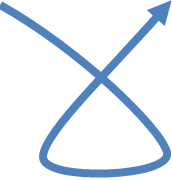
\includegraphics[width=10pt]{img/prodcroix} & v_3 \\
u_1 & 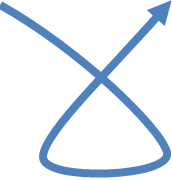
\includegraphics[width=10pt]{img/prodcroix}& v_1 \\
u_2 & 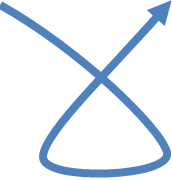
\includegraphics[width=10pt]{img/prodcroix}& v_2
\end{array}
\right]$}{}
\end{minipage}
}}

{\frame{
\frametitle{Produit mixte}

\begin{defi}
Soient trois vecteurs $\overrightarrow{u}$, $\overrightarrow{v}$, $\overrightarrow{w}$, le produit mixte revient à calculer:
$\left[\overrightarrow{u},\overrightarrow{v},\overrightarrow{w}\right]=(\overrightarrow{u}\wedge \overrightarrow{v}).\overrightarrow{w}$
\end{defi}

Ainsi:

\begin{itemize}
 \item $\left[\overrightarrow{u},\overrightarrow{v},\overrightarrow{w}\right]=\left[\overrightarrow{v},\overrightarrow{w},\overrightarrow{u}\right]=\left[\overrightarrow{w},\overrightarrow{u},\overrightarrow{v}\right]$,
 \item $\left[\overrightarrow{v},\overrightarrow{u},\overrightarrow{w}\right]=\left[\overrightarrow{w},\overrightarrow{v},\overrightarrow{u}\right]=\left[\overrightarrow{u},\overrightarrow{w},\overrightarrow{v}\right]=-\left[\overrightarrow{u},\overrightarrow{v},\overrightarrow{w}\right]$,
 \item $\left[\overrightarrow{u},\overrightarrow{v},\overrightarrow{w}\right]=\left[ \begin{array}{ccc}
 u_x & u_y & u_z \\
 v_x & v_y & v_z \\
 w_x & w_y & w_z
 \end{array}\right]$
 \item $\left[\overrightarrow{u},\overrightarrow{v},\overrightarrow{w}\right]=(u_x v_y w_z + v_x w_y u_z + w_x u_y v_z) - (w_x v_y u_z + v_x u_y w_z + u_x w_y v_z)$
\end{itemize}

Si deux des trois vecteurs sont égaux ou colinéaires, le produit mixte est nul.

Si les vecteurs $\overrightarrow{u}$, $\overrightarrow{v}$ et $\overrightarrow{w}$ ont même origine, la valeur absolue du produit mixte $\left[\overrightarrow{u},\overrightarrow{v},\overrightarrow{w}\right]$, est égale au volume du parallélépipède construit sur $\overrightarrow{u}$, $\overrightarrow{v}$ et $\overrightarrow{w}$.
}}

{\frame{
\frametitle{Double produit vectoriel}

\begin{itemize}
 \item Combiner trois vecteurs $\overrightarrow{u}$, $\overrightarrow{v}$ et $\overrightarrow{w}$ par deux produits vectoriels successifs permet d'obtenir un double produit vectoriel, \vfill
 \item Exemple: $\overrightarrow{u}\wedge (\overrightarrow{v} \wedge \overrightarrow{w})$, \vfill
 \item Attention: comme le produit vectoriel n'est ni associatif, ni commutatif, il est nécessaire d'utiliser comme ici des parenthèses et le résultat va dépendre à la fois de l'ordre dans lequel les opérations sont effectuées et de l'ordre de présentation des 3 vecteurs, \vfill
 \item Les 2 formules suivantes peuvent être démontrées: \\ 
$\overrightarrow{u}\wedge (\overrightarrow{v}\wedge \overrightarrow{w})=(\overrightarrow{u}.\overrightarrow{w})\overrightarrow{v}-(\overrightarrow{u}.\overrightarrow{v})\overrightarrow{w}$ \\
$(\overrightarrow{u}\wedge \overrightarrow{v})\wedge \overrightarrow{w}=(\overrightarrow{u}.\overrightarrow{w})\overrightarrow{v}-(\overrightarrow{v}.\overrightarrow{w})\overrightarrow{u}$ 
\end{itemize}
}}

\section{Champ de vecteur et torseur}

{\frame{
\frametitle{Champ de vecteurs}

Un champ de vecteurs est une application qui définit un vecteur $\overrightarrow{V_M}$ en tout point de l'espace (champ de vecteurs vitesse, champ magnétique, champ de pesanteur,...),

\vfill

\begin{defi}
Un champ de vecteurs $\overrightarrow{M_P}$ équiprojectif est un champ de vecteurs qui répond au théorème de Varignon (parfois appelé théorème de BABAR \og entre nous \fg).

\begin{center}
\ifdef{\public}{$\overrightarrow{M_B}=\overrightarrow{M_A}+\overrightarrow{BA}\wedge \overrightarrow{R}$}{}
\end{center}

\begin{itemize}
 \item $\overrightarrow{R}$ est un vecteur caractéristique du champ de vecteurs appelé « résultante » 
 \item $\overrightarrow{M_P}$ sont les moments en chaque point P du champ de vecteurs. 
\end{itemize}
\end{defi}
}}

{\frame{
\frametitle{L'équiprojectivité}

\begin{minipage}{0.6\linewidth}
\begin{defi}
La propriété d'équiprojectivité d'un tel champ de vecteurs est exprimée par le fait que deux moments $\overrightarrow{M_A}$ et $\overrightarrow{M_B}$ du champ de vecteurs ont la même projection sur la droite passant par les deux points A et B : 
$\overrightarrow{AA'}=\overrightarrow{BB'}$
\end{defi}
\end{minipage}
\hfill
\begin{minipage}{0.35\linewidth}
 \centering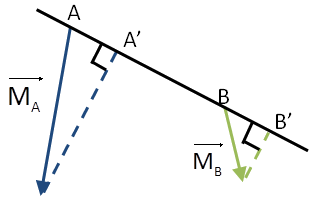
\includegraphics[width=0.7\linewidth]{img/vecteur5}
\end{minipage}

\vfill

\textit{Démonstration:}
En partant du théorème de Varignon et en multipliant par $\overrightarrow{AB}$, on obtient 

$\overrightarrow{M_B}.\overrightarrow{AB}=\overrightarrow{M_A}.\overrightarrow{AB}+(\overrightarrow{BA}\wedge \overrightarrow{R}).\overrightarrow{AB}$ or $(\overrightarrow{BA}\wedge \overrightarrow{R}).\overrightarrow{AB}=0$
donc $AA'=BB'$.

\vfill

Remarques:
\begin{itemize}
 \item La distribution des vecteurs vitesse dans un solide indéformable est un champ de vecteurs équiprojectif puisque il respecte le théorème de Varignon,
 \item L'équiprojectivité entre les vecteurs vitesse peut, donc, être utilisée pour les constructions graphiques. 
\end{itemize}
}}


{\frame{
\frametitle{Le torseur}

Un torseur est la représentation d'un champ de vecteurs équiprojectif, dont les vecteurs $\overrightarrow{M_P}$ en chaque point P s'appellent \og moments \fg du torseur. De par les propriétés d'un tel champ, les moments en deux points P et O vérifient la relation de Varignon.

\vfill

\begin{defi}
\textit{Éléments de réduction d'un torseur} \\
Un torseur est donc déterminé par deux vecteurs, constituant sa \og réduction \fg en un point quelconque P de l'espace, à savoir : 
\begin{itemize}
 \item La résultante $\overrightarrow{R}$, ce vecteur est unique et indépendant du point de réduction,
 \item Le moment en P du torseur $\overrightarrow{M_P}$.
\end{itemize}
\end{defi}

\vfill

\begin{minipage}{0.46\linewidth}
\textit{Remarque:} La résultante est donc un vecteur caractéristique du champ qui permet, à partir du moment en un point particulier, de retrouver les autres moments
\end{minipage}\hfill
\begin{minipage}{0.50\linewidth}
\begin{center}
\ifdef{\public}{\begin{math}
	 \left\{T \right\}_P=\left\{ \begin{array}{c} \overrightarrow{R} \\ \overrightarrow{M_P} \end{array}\right\}_P=
	 \left\{ \begin{array}{cc} \theta_x & x \\ \theta_y & y \\ \theta_z & z \end{array}\right\}_{P,R(\overrightarrow{x},\overrightarrow{y},\overrightarrow{z})}
	\end{math}}{\vspace{20pt}}
\end{center}
\end{minipage}

}}


{\frame{
\frametitle{Invariants d'un torseur}

Un torseur possède deux grandeurs indépendantes du point où on l'écrit:
\begin{itemize}
 \item l'invariant vectoriel : la résultante $\overrightarrow{R}$,
 \item l'invariant scalaire appelé aussi l'automoment: $A=\overrightarrow{R}.\overrightarrow{M_A}=\overrightarrow{R}.\overrightarrow{M_B}$
\end{itemize}

\vfill

Torseurs particuliers
\begin{itemize}
 \item Le torseur à résultante ou glisseur est un torseur dont:
\begin{itemize}
 \item l'automoment est nul, c'est à dire que le résultante et le moment sont orthogonaux en tout points
 \item le moment est nul en tout point de de son axe. 
\end{itemize}
 \item Le torseur couple est un torseur dont la résultante est nulle. 
\end{itemize}
}}

{\frame{
\frametitle{Opérations sur les torseurs}

\begin{itemize}
 \item Égalité de deux torseurs \\ \vspace{10pt}
 \begin{math}
 \left\{T_1\right\}_O=\left\{\begin{array}{c} \overrightarrow{R_1} \\ \overrightarrow{M_1} \end{array}\right\}_O=
 \left\{T_2\right\}_O=\left\{\begin{array}{c} \overrightarrow{R_2} \\ \overrightarrow{M_2} \end{array}\right\}_O
 \rightarrow \overrightarrow{R_1}=\overrightarrow{R_2}, \overrightarrow{M_1}=\overrightarrow{M_2}
 \end{math}
 \item Somme de deux torseurs \\ \vspace{10pt}
 \begin{math}
 \left\{T_1\right\}_O+\left\{T_2\right\}_O=\left\{\begin{array}{c} \overrightarrow{R_1} \\ \overrightarrow{M_1} \end{array}\right\}_O + \left\{\begin{array}{c} \overrightarrow{R_2} \\ \overrightarrow{M_2} \end{array}\right\}_O
 =\left\{\begin{array}{c} \overrightarrow{R_1}+\overrightarrow{R_2} \\ \overrightarrow{M_1}+\overrightarrow{M_2} \end{array}\right\}_O
 \end{math}
 \item Multiplication d'un torseur par un scalaire \\ \vspace{10pt}
 \begin{math}
 \lambda.\left\{T_1\right\}_O=\left\{\begin{array}{c} \lambda.\overrightarrow{R_1} \\ \lambda.\overrightarrow{M_1} \end{array}\right\}_O
 \end{math}
\end{itemize}
}}

{\frame{
\frametitle{Éléments centraux d'un torseur}

\begin{itemize}
 \item Point central \\ \vspace{10pt} 
Un point central d'un torseur est un point pour lequel la résultante et le moment sont colinéaires : 

Si $\overrightarrow{M_P}=\lambda.\overrightarrow{R}$ alors P est un point central, en P, le moment du torseur est minimum. 

\hfill

 \item Détermination de l'axe central \\ \vspace{10pt}
Soit un torseur $\left\{T\right\}_O=\left\{\begin{array}{c} \lambda.\overrightarrow{R} \\ \lambda.\overrightarrow{M} \end{array}\right\}_O$

L'axe central du torseur est la droite parallèle à $\overrightarrow{R}$ et passant par le point P tel que : \\ \vspace{10pt} $\overrightarrow{OP}=\frac{\overrightarrow{R}\wedge\overrightarrow{M_O}}{\overrightarrow{R}^2}$

\end{itemize}
}}


\section{Repères de projection}

{\frame{
\frametitle{Les repères de projection}

\begin{minipage}{0.78\linewidth}
	\begin{itemize}
	 \item Les opérations sur les torseurs et les vecteurs présentées ci-dessus ne sont valables que si ces éléments sont présentés sur le même repère.
	 \item Il sera souvent utile dans le cas d'une résolution de cinématique d'introduire plusieurs repères.
	 \item Ainsi, la suite montre les méthodes pour ramener les torseurs et les vecteurs dans le même repère de description.
	 \item Cas 1: Un repère global
	  \begin{itemize}
	   \item $R_0$: Lié à la pièce $0$: $\overrightarrow{AC}=\overrightarrow{AB}+\overrightarrow{BC}=a_1.\overrightarrow{x_0}+a_2.\overrightarrow{y_0}+b_1.\overrightarrow{x_0}+b_2.\overrightarrow{y_0}$,
	   \item $a_i$ et $b_i$ sont des variables en fonction du déplacement des pièces.
	  \end{itemize}
	 \item Cas 2: Un repère associé à chaque pièce
	 \begin{itemize}
	  \item $R_0$: Lié à la pièce $0$, $R_1$: Lié à la pièce $1$, $R_2$: Lié à la pièce $2$. $\overrightarrow{AC}=\overrightarrow{AB}+\overrightarrow{BC}=a_1.\overrightarrow{x_1}+b_1.\overrightarrow{x_2}$
	   \item $a_i$ et $b_i$ sont des constantes liées aux dimensions des pièces.
	 \end{itemize}
	\end{itemize}
\end{minipage}
 \hfill
\begin{minipage}{0.17\linewidth}
	\centering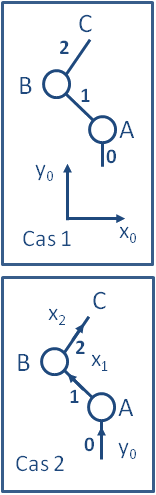
\includegraphics[width=\linewidth]{img/repere4}
\end{minipage}
}}

{\frame{
\frametitle{Changement de repère dans les espaces affines}

\begin{itemize}
 \item Soient $R=(O,e)$ et $R'=(O',e')$ deux repères différents, alors les coordonnées.

$\overrightarrow{M_{R'}}=\left(\begin{array}{c} x' \\ y' \\ z' \end{array}\right)$ s'obtiennent à partir des coordonnées 
$\overrightarrow{M_R}=\left(\begin{array}{c} x \\ y \\ z \end{array}\right)$ du même point $M$ mais dans le repère $R$, à l'aide de 3 équations:

\begin{flushright}
\begin{math}
\left\{ \begin{array}{l} \ifdef{\public}{x'=a_{11}.x+a_{12}.y+a_{13}.z \\ y'=a_{21}.x+a_{22}.y+a_{23}.z \\ z'=a_{31}.x+a_{32}.y+a_{33}.z}{ ..................................\\ .................................. \\  ..................................}
\end{array}\right.
\end{math}
\end{flushright} \vfill
 \item Matriciellement ces équations s'écrivent: $M_{R'}=A.M_R+B$ où $A=(a_{ij})_{1\leq i,j \leq 3}$ est la matrice de passage dans V.
\end{itemize}
}}

{\frame{
\frametitle{Changement d'axes de coordonnées}

\begin{itemize}
 \item Les formules qui suivent permettent d'exprimer les coordonnées d'un point M dans l'un des repères en fonction des coordonnées dans l'autre repère, \vfill
 \item Soit un repère cartésien $O(\overrightarrow{x},\overrightarrow{y})$ dans lequel les coordonnées $(x,y)$ d'un point M s'expriment en fonction des coordonnées polaires $(r,\phi)$ par les formules élémentaires
 
 \begin{center}
 $\left\{ \begin{array}{l}  \ifdef{\public}{x=r.cos(\phi) \\ y=r.sin(\phi)}{..................................\\ ..................................} \end{array}  \right.$
 \end{center} \vfill
\item Dans le nouveau repère $O(\overrightarrow{x'},\overrightarrow{y'})$ déduit du précédent par une rotation d'angle $\theta$ les nouvelles coordonnées polaires sont $r$ et $(\phi-\theta)$ et les coordonnées cartésiennes deviennent:

 \begin{center}
 $\left\{ \begin{array}{l} \ifdef{\public}{x'=r.cos(\phi-\theta) \\ y'=r.sin(\phi-\theta)}{..................................\\ ..................................} \end{array}  \right.$
 \end{center}
\end{itemize}
}}

{\frame{
\frametitle{Changement d'axes de coordonnées}

\begin{minipage}{0.65\linewidth}
\begin{defi}
\begin{itemize}
 \item Les formules suivantes permettant de passer d'un repère à l'autre.

$\left\{\begin{array}{l} \ifdef{\public}{\overrightarrow{x'}=cos(\theta).\overrightarrow{x}+sin(\theta).\overrightarrow{y} \\ \overrightarrow{y'}=-sin(\theta).\overrightarrow{x}+cos(\theta).\overrightarrow{y}}{.............................................\\ .............................................}\end{array}\right.$
 \item En sens inverse,

$\left\{\begin{array}{l} \ifdef{\public}{\overrightarrow{x}=cos(\theta).\overrightarrow{x'}-sin(\theta).\overrightarrow{y'} \\ \overrightarrow{y}=sin(\theta).\overrightarrow{x'}+cos(\theta).\overrightarrow{y'}}{.............................................\\ .............................................}\end{array}\right.$
\end{itemize}
\vspace{-10pt}\end{defi}
\end{minipage}
 \hfill
\begin{minipage}{0.31\linewidth}
	\centering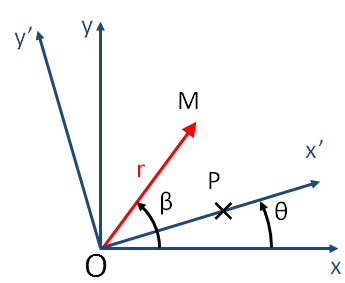
\includegraphics[width=\linewidth]{img/repere5}
\end{minipage}

\vfill

Remarque : s'il peut s'avérer difficile de mémoriser le signe à mettre devant $sin(\theta)$ ($+$ dans une ligne et $-$ dans l'autre) l'astuce consiste à considérer un point particulier (tel que P sur la figure) avec $y=0$ ou $y'=0$ selon les besoins et de vérifier alors sur la figure le signe de la coordonnée voulue.
}}


{\frame{
\frametitle{Application}

Exemple de pièce munie de deux repères $R(O,\overrightarrow{x},\overrightarrow{y},\overrightarrow{z})$ et $R_1(O,\overrightarrow{x_1},\overrightarrow{y_1},\overrightarrow{z_1})$

\begin{center}
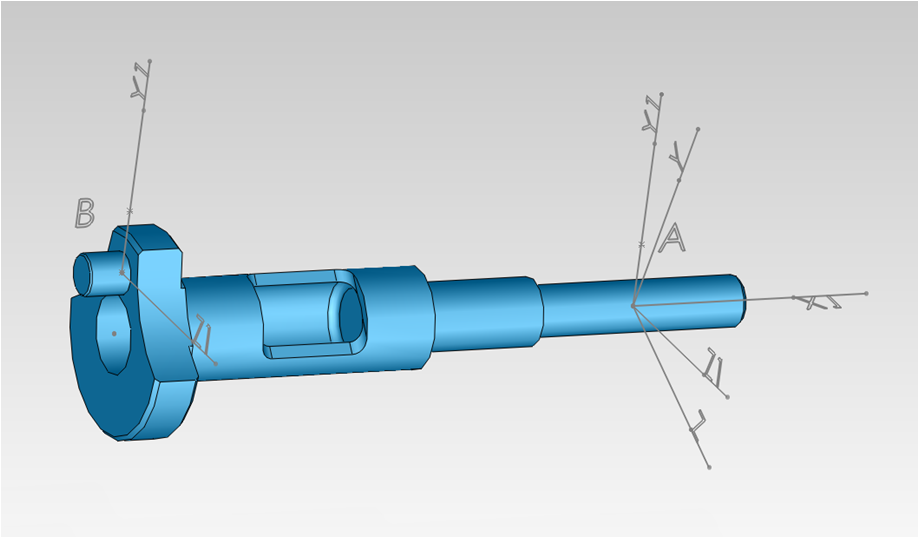
\includegraphics[width=0.9\linewidth]{img/villebrequin1}
\end{center}
}}

{\frame{
\frametitle{Projection de vecteurs dans une base}

\begin{minipage}{0.48\linewidth}
Soit $\theta$, l'angle entre $Z$ et $Z_1$, écrire les coordonnées du vecteur $\overrightarrow{AB}$, dans les deux repères (choisir les inconnues nécessaires).
\end{minipage}
\hfill
\begin{minipage}{0.48\linewidth}
\centering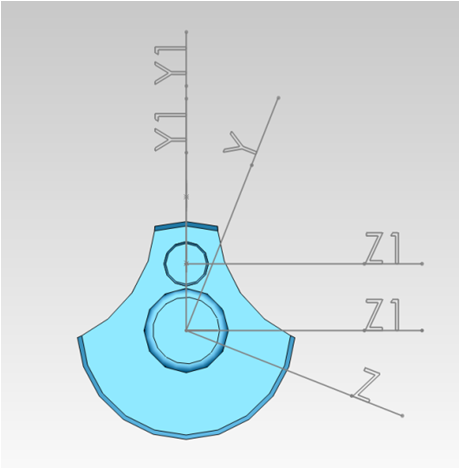
\includegraphics[width=0.8\linewidth]{img/villebrequin2}
\end{minipage}

\vfill

\begin{minipage}{0.48\linewidth}
Ainsi, les coordonnées d'un vecteur varient selon qu'elles sont écrites dans le repère local ou le repère global.
\end{minipage}
\hfill
\begin{minipage}{0.48\linewidth}
\centering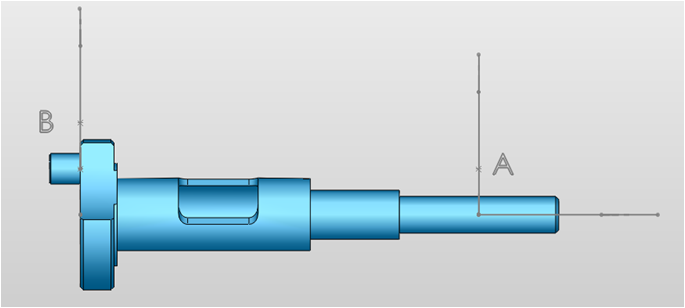
\includegraphics[width=0.8\linewidth]{img/villebrequin3}
\end{minipage}
}}

{\frame{
\frametitle{Conclusion}

\begin{savoir}
Vous devez être capable de:
\begin{itemize}
 \item définir un vecteur à partir de sa \textbf{direction}, de son \textbf{sens} et de sa \textbf{norme},
 \item projeter des vecteurs dans une base,
 \item faire un produit scalaire,
 \item faire un produit vectoriel,
 \item décrire un champ de vecteur avec un torseur,
 \item manipuler les éléments de réduction du torseur,
 \item modifier le repère de projection d'un vecteur.
\end{itemize}
\end{savoir}
}}


\end{document}

{\frame{
\frametitle{Torseurs classiques}

Les torseurs classiques sont définis en connaissant les mouvements autorisés et les degrés de liberté de la liaison.

\begin{center}
\begin{tabular}{|m{3cm}|c|m{3cm}|}
\hline
Liaison pivot & Torseur cinématique & Axes nécessaires \\
 & $\left\{ \begin{array}{cc} \theta_x & 0 \\ 0 & 0 \\ 0 & 0 \end{array}\right\}_{O}$  & 1 axe $\overrightarrow{x}$\\
\hline
Liaison glissière & Torseur cinématique & Axes nécessaires \\
 & $\left\{ \begin{array}{cc} 0 & x \\ 0 & 0 \\ 0 & 0 \end{array}\right\}_{O}$  & 1 axe $\overrightarrow{x}$\\
\hline
Liaison hélicoïdale & Torseur cinématique & Axes nécessaires \\
 & $\left\{ \begin{array}{cc} \theta_x & x \\ 0 & 0 \\ 0 & 0 \end{array}\right\}_{O}$  & \begin{tabular}{l} 1 axe $\overrightarrow{x}$ \\ $x=\frac{p.\theta_x}{2\pi}$ \end{tabular} \\
\hline
\end{tabular}
\end{center}
}}

{\frame{
\frametitle{Torseurs classiques}

\begin{center}
\begin{tabular}{|m{3cm}|c|m{3cm}|}
\hline
Liaison pivot glissant & Torseur cinématique & Axes nécessaires \\
 & $\left\{ \begin{array}{cc} \theta_x & x \\ 0 & 0 \\ 0 & 0 \end{array}\right\}_{O}$  & 1 axe $\overrightarrow{x}$\\
\hline
Liaison sphérique à doigts & Torseur cinématique & Axes nécessaires \\
 & $\left\{ \begin{array}{cc} \theta_x & 0 \\ \theta_y & 0 \\ 0 & 0 \end{array}\right\}_{O}$  & 0 axe \\
\hline
Liaison sphérique ou rotule & Torseur cinématique & Axes nécessaires \\
 & $\left\{ \begin{array}{cc} \theta_x & 0 \\ \theta_y & 0 \\ \theta_z & 0 \end{array}\right\}_{O}$  & 0 axe \\
\hline
Liaison appui plan & Torseur cinématique & Axes nécessaires \\
 & $\left\{ \begin{array}{cc} 0 & x \\ 0 & y \\ \theta_z & 0 \end{array}\right\}_{O}$  & \begin{tabular}{l} 1 axe $\overrightarrow{z}$ \\ normale au plan \end{tabular} \\
\hline
\end{tabular}
\end{center}
}}

{\frame{
\frametitle{Torseurs classiques}

\begin{center}
\begin{tabular}{|m{3cm}|c|m{3cm}|}
\hline
Liaison linéaire annulaire & Torseur cinématique & Axes nécessaires \\
 & $\left\{ \begin{array}{cc} \theta_x & x \\ \theta_y & 0 \\ \theta_z & 0 \end{array}\right\}_{O}$  & 1 axe $\overrightarrow{x}$\\
\hline
Liaison linéaire rectiligne & Torseur cinématique & Axes nécessaires \\
 & $\left\{ \begin{array}{cc} \theta_x & x \\ 0 & y \\ \theta_z & 0 \end{array}\right\}_{O}$  & \begin{tabular}{l} 2 axes $\overrightarrow{x}$, $\overrightarrow{z}$ \\ direction de la ligne $\overrightarrow{x}$ \\ normale au plan $\overrightarrow{z}$ \end{tabular} \\
\hline
Liaison linéaire ponctuelle & Torseur cinématique & Axes nécessaires \\
 & $\left\{ \begin{array}{cc} \theta_x & x \\ \theta_y & y \\ \theta_z & 0 \end{array}\right\}_{O}$  & \begin{tabular}{l} 1 axe $\overrightarrow{z}$ \\ normale au plan \end{tabular} \\
\hline
Liaison encastrement & Torseur cinématique & Axes nécessaires \\
 & $\left\{ \begin{array}{cc} 0 & 0 \\ 0 & 0 \\ 0 & 0 \end{array}\right\}_{O}$  & 0 axe \\
\hline
\end{tabular}
\end{center}
}}





